% Created 2021-09-26 Sun 10:55
% Intended LaTeX compiler: pdflatex
\documentclass[letter]{article}
\usepackage[utf8]{inputenc}
\usepackage[T1]{fontenc}
\usepackage{graphicx}
\usepackage{grffile}
\usepackage{longtable}
\usepackage{wrapfig}
\usepackage{rotating}
\usepackage[normalem]{ulem}
\usepackage{amsmath}
\usepackage{textcomp}
\usepackage{amssymb}
\usepackage{capt-of}
\usepackage{hyperref}
\usepackage{multicol}
\usepackage[margin=1.3in]{geometry}
\setlength{\columnsep}{1cm}
\usepackage{palatino}
\fontfamily{ppl}\selectfont
\usepackage[spanish, es-noindentfirst]{babel}
\usepackage{setspace}
\setstretch{1.5}
\usepackage{fancyhdr}
\fancyhf{}
\pagestyle{fancy}
\lhead{\hleft}
\rhead{\hright}
\cfoot{\thepage}
\renewcommand{\headrulewidth}{1pt}
\renewcommand{\footrulewidth}{0pt}
\newcommand{\hleft}{Primer examen parcial}
\newcommand{\hright}{Jesus Rodolfo Izurieta Veliz}
\author{Jesus Rodolfo Izurieta Veliz}
\date{\today}
\title{Primer examen parcial - INF 354}
\hypersetup{
 pdfauthor={Jesus Rodolfo Izurieta Veliz},
 pdftitle={Primer examen parcial - INF 354},
 pdfkeywords={},
 pdfsubject={},
 pdfcreator={Emacs 27.2 (Org mode 9.5)}, 
 pdflang={Spanish}}
\begin{document}

\maketitle


\section{Introducción}
\label{sec:org50bc9ee}

\subsection{Selección del dataset}
\label{sec:org04add11}

El dataset seleccionado para la realización práctica de la prueba, muestra datos
de mediciones de signos relacionadas a apoplejías o \textbf{accidente cerebrovascular}, con la
finalidad de poder predecir, según estos indicadores, si una persona es propensa
a sufrir este padecimiento.

Según la Organización Mundial de la Salud (OMS), el accidente cerebrovascular es
la segunda causa principal de muerte a nivel mundial, responsable de
aproximadamente el 11 \% del total de muertes. Este conjunto de datos se utiliza
para predecir si es probable que un paciente contraiga un accidente
cerebrovascular en función de los parámetros de entrada como el sexo, la edad,
varias enfermedades y el estado tabáquico. Cada fila de los datos proporciona
información relevante sobre el paciente.

El dataset está públicamente disponible en la dirección: \url{https://www.kaggle.com/fedesoriano/stroke-prediction-dataset}

\subsubsection{Información de atributos}
\label{sec:orgdb6629a}

\begin{enumerate}
\item \texttt{id}: identificador único
\item \texttt{gender}: \guillemotleft{}\texttt{Male}\guillemotright{}, \guillemotleft{}\texttt{Female}\guillemotright{} u \guillemotleft{}\texttt{Other}\guillemotright{}
\item \texttt{age}: edad del paciente
\item \texttt{hipertenssion}: 0 si el paciente no tiene hipertensión, 1 si el paciente tiene hipertensión
\item \texttt{heart\_disease}: 0 si el paciente no tiene ninguna enfermedad cardíaca, 1 si el paciente tiene una enfermedad cardíaca
\item \texttt{ever\_married}: \guillemotleft{}\texttt{No}\guillemotright{} o \guillemotleft{}\texttt{Yes}\guillemotright{}
\item \texttt{work\_type}: \guillemotleft{}\texttt{children}\guillemotright{}, \guillemotleft{}\texttt{Govt\_jov}\guillemotright{}, \guillemotleft{}\texttt{Never\_worked}\guillemotright{}, \guillemotleft{}\texttt{Private}\guillemotright{} o \guillemotleft{}\texttt{Self-employed}\guillemotright{}
\item \texttt{Residence\_type}: \guillemotleft{}\texttt{Rural}\guillemotright{} o \guillemotleft{}\texttt{Urban}\guillemotright{}
\item \texttt{avg\_grucose\_level}: nivel promedio de glucosa en la sangre
\item \texttt{bmi}: índice de masa corporal
\item \texttt{smoking\_status}: \guillemotleft{}\texttt{formerly smoked}\guillemotright{}, \guillemotleft{}\texttt{never smoked}\guillemotright{}, \guillemotleft{}\texttt{smokes}\guillemotright{} o \guillemotleft{}\texttt{unknown}\guillemotright{}*
\item \texttt{stroke}: 1 si el paciente tuvo un accidente cerebrovascular o 0 si no
\end{enumerate}

*Nota: \guillemotleft{}Unknown\guillemotright{} en \texttt{smoking\_status} significa que la información no está disponible para este paciente.

\begin{figure}[htbp]
\centering
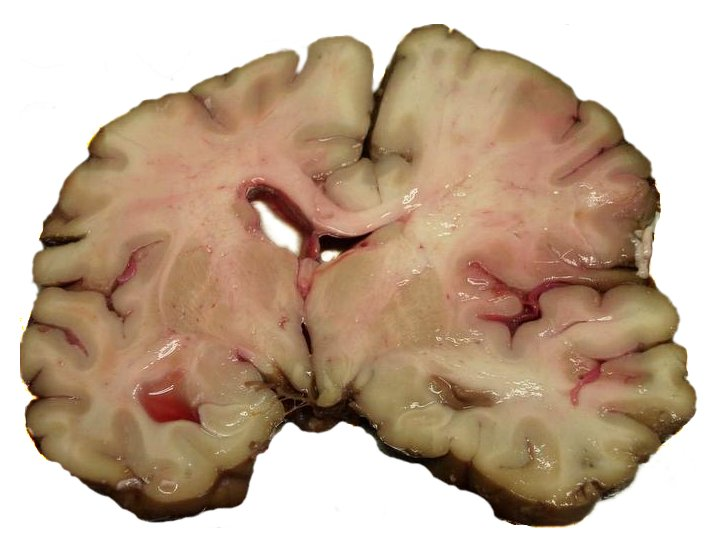
\includegraphics[width=200px]{./img/stroke.jpg}
\caption{Sección de cerebro procedente de un difunto que sufrió un ataque cerebrovascular (ACV) a nivel de la arteria cerebral media.}
\end{figure}

\section{Desarrollo}
\label{sec:org5877377}

El desarrollo de las preguntas del examen se realizó en anaconda, este documento
presenta parte del desarrollo, el código completo se encuentra en los
repositorios específicos de cada pregunta.

\subsection{Pregunta 1}
\label{sec:org2bf42d2}

Dirección del repositorio: \url{https://github.com/izurietajr/primer-parcial-354-1}

Seleccione un dataset de los propuestos por su persona en una anterior tarea, esta debe ser tabular de al menos 1000 filas y 5 columnas. Realice lo siguiente:

\begin{enumerate}
\item La media, moda y la desviación estándar por columna; explique qué significa en cada caso mediante Python sin uso de librerías
\item La media, la moda, la desviación estándar con el uso de numpy y pandas
\item Grafique los datos y explique su comportamiento (PYTHON)
\end{enumerate}

\subsubsection{Media, moda y desviación estándar (Python)}
\label{sec:org5f37919}

\textbf{Cargado de los datos}

Usaremos la función open de python para abrir el archivo del dataset en formato csv y crearemos una estructura orientada a objetos para facilitar el manejo de nuestro dataset.

\begin{verbatim}
class Dataset:
    def __init__(self, url):
        self.load_csv(url)

    def load_csv(self, url):
        content = []
        with open(url) as file:
            lines = file.readlines()
            for line in lines:
                line = line.replace("\n", "")
                content.append(line.split(","))
        self.headers, self.data = content[0], content[1:]
        return self.headers, self.data

    def get_column(self, column):
        index = self.headers.index(column)
        try:
            return [float(x[index]) for x in self.data]
        except Exception as e:
            print(e)
            return []

dataset = Dataset("stroke-dataset.csv")

print(dataset.headers)
print(dataset.data[:3])
\end{verbatim}

Mostramos los nombres de los campos obtenidos del archivo csv y las primeras
tres líneas de datos, la salida de la ejecución muestra:

\texttt{['id', 'gender', 'age', 'hypertension', 'heart\_disease', 'ever\_married', 'work\_type', 'Residence\_type', 'avg\_glucose\_level', 'bmi', 'smoking\_status', 'stroke']}

\texttt{[['9046', 'Male', '67', '0', '1', 'Yes', 'Private', 'Urban', '228.69', '36.6', 'formerly smoked', '1'], ['51676', 'Female', '61', '0', '0', 'Yes', 'Self-employed', 'Rural', '202.21', 'N/A', 'never smoked', '1'], ['31112', 'Male', '80', '0', '1', 'Yes', 'Private', 'Rural', '105.92', '32.5', 'never smoked', '1']]}

Los nombres de los campos se nos muestran como una lista de cadenas, mientras
que los datos se encuentran en una matriz (lista de listas) donde cada línea
corresponde a una lista dentro de la lista \texttt{data}.

\textbf{Cálculo de la media}

La media muestral es calculada bajo la siguiente definición, considerando que se tiene una muestra \((X_1, X_2, ..., X_n)\):

$$
\bar X_n = \frac{1}{n}\sum_{i=1}^{n}{X_i} = \frac{X_1+X_2+...+X_n}{n}
$$

\begin{verbatim}
def media(lista):
    if lista != []:
        suma = sum(lista)
        return suma/len(lista)
    else:
        return None

age = dataset.get_column("age")
media(age)
\end{verbatim}

Como resultado se muestra:

\texttt{43.226614481409015}

\textbf{Cálculo de la moda}

La moda es el valor más común en cuanto a frecuencia, por lo que para
calcularla, obtendremos la frecuencia de cada ocurrencia y seleccionaremos la
mayor.

\begin{verbatim}
from functools import reduce

def moda(lista):
    freq = {}
    for i in lista:
        if i not in freq:
            freq[i] = 1
        else:
            freq[i] = freq[i]+1
    items = [(r, s) for r, s in freq.items()]
    moda = reduce(lambda x, y: x if x[1] > y[1] else y, items)
    return moda[0]

moda(age)
\end{verbatim}

Dando como resultado:

\begin{verbatim}
78.0
\end{verbatim}

\textbf{Cálculo de la desviación estándar}

La desviación estándar de una población estadística, conjunto de datos o
distribución de probabilidad es la raíz cuadrada de su varianza, que es una
medida de dispersión definida como la esperanza del cuadrado de la desviación de
dicha variable respecto a su media.

\begin{verbatim}
from math import sqrt

def sd(lista):
    media_ = media(lista)
    smt = [(i-media_)**2 for i in lista]
    return sqrt(media(smt))

sd(age)
\end{verbatim}

Dando como resultado:

\begin{verbatim}
22.61043402711301
\end{verbatim}

\subsubsection{Media, moda y desviación estándar (Numpy, Pandas)}
\label{sec:orgfea8baa}

\textbf{Cargado de datos}

Usaremos la librería pandas para leer el archivo csv y así poder obtener el dataset.

\begin{verbatim}
import pandas as pd
import numpy as np
from scipy import stats as st

data = pd.read_csv("stroke-dataset.csv")
print(data)
\end{verbatim}

Nos mostrará parte del dataset:

\begin{verbatim}
         id  gender   age  hypertension  heart_disease ever_married  \
0      9046    Male  67.0             0              1          Yes
1     51676  Female  61.0             0              0          Yes
2     31112    Male  80.0             0              1          Yes
3     60182  Female  49.0             0              0          Yes
4      1665  Female  79.0             1              0          Yes
...     ...     ...   ...           ...            ...          ...
5105  18234  Female  80.0             1              0          Yes
5106  44873  Female  81.0             0              0          Yes
5107  19723  Female  35.0             0              0          Yes
5108  37544    Male  51.0             0              0          Yes
5109  44679  Female  44.0             0              0          Yes

          work_type Residence_type  avg_glucose_level   bmi   smoking_status  \
0           Private          Urban             228.69  36.6  formerly smoked
1     Self-employed          Rural             202.21   NaN     never smoked
2           Private          Rural             105.92  32.5     never smoked
3           Private          Urban             171.23  34.4           smokes
4     Self-employed          Rural             174.12  24.0     never smoked
...             ...            ...                ...   ...              ...
5105        Private          Urban              83.75   NaN     never smoked
5106  Self-employed          Urban             125.20  40.0     never smoked
5107  Self-employed          Rural              82.99  30.6     never smoked
5108        Private          Rural             166.29  25.6  formerly smoked
5109       Govt_job          Urban              85.28  26.2          Unknown

      stroke
0          1
1          1
2          1
3          1
4          1
...      ...
5105       0
5106       0
5107       0
5108       0
5109       0

[5110 rows x 12 columns]
\end{verbatim}

\textbf{Cálculo de la media, moda y desviación estándar}

Para calcular estos estadísticos, usaremos la librería numpy.

\begin{verbatim}
np.mean(data['age'])
\end{verbatim}

salida:

\begin{verbatim}
43.226614481409015
\end{verbatim}

Ya que numpy no provee un método para calcular la moda, usaremos la librería scipy, importaremos el módulo stats de esta, que provee la función mode.

\begin{verbatim}
st.mode(data['age'])
\end{verbatim}

salida:

\begin{verbatim}
ModeResult(mode=array([78.]), count=array([102]))
\end{verbatim}

Desviación estándar:

\begin{verbatim}
np.std(data['age'])
\end{verbatim}

salida:

\begin{verbatim}
22.61043402711301
\end{verbatim}

Como podemos ver, los valores calculados con las librerías de python, coinciden con los valores calculados previamente.

\subsubsection{Gráficas e interpretación de datos}
\label{sec:orgabae004}

Usaremos la librería matplotlib para hacer gráficos con los datos del dataset.

\begin{verbatim}
import matplotlib.pyplot as plt

strokes = data[data.stroke == 1]
strokes.head()
\end{verbatim}

\begin{center}
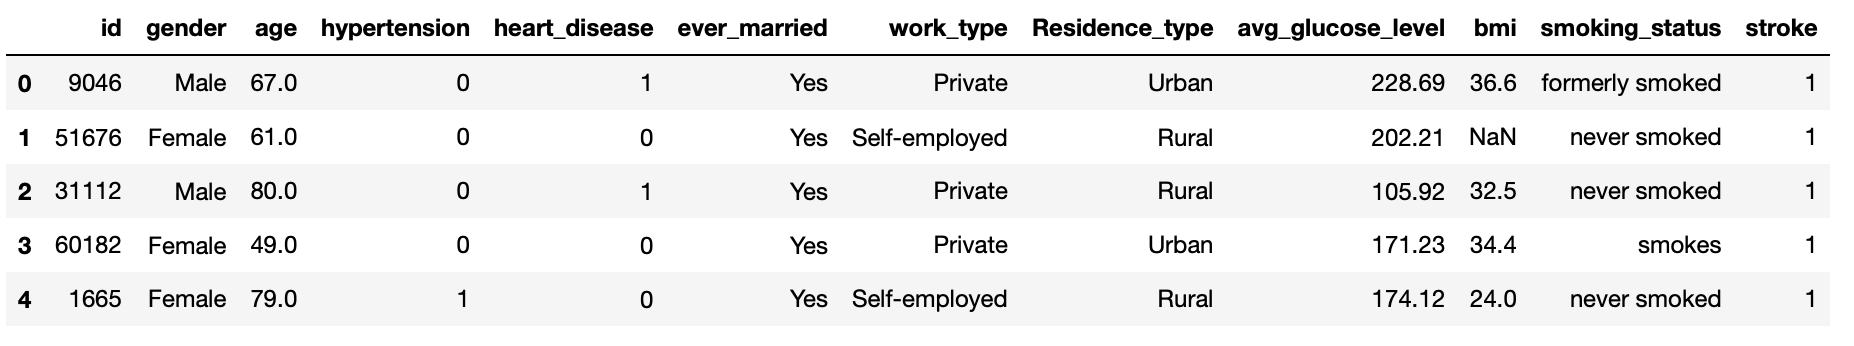
\includegraphics[width=.9\linewidth]{./img/tabla.png}
\end{center}

Realizamos el gráfico de un histograma de la siguiente manera:

\begin{verbatim}
hist, edges = np.histogram(data['age'])

plt.plot(hist)
\end{verbatim}

Con esto, obtenemos el gráfico:

\begin{center}
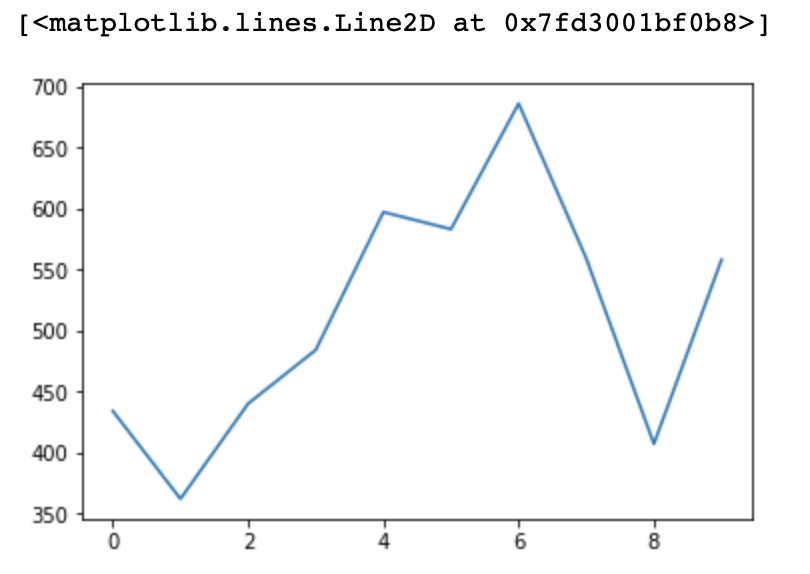
\includegraphics[width=.9\linewidth]{./img/hist.png}
\end{center}

\subsection{Pregunta 2}
\label{sec:org4178403}

Dirección del repositorio: \url{https://github.com/izurietajr/primer-parcial-354-2}

\section{Referencias}
\label{sec:orgf1e5609}

\url{https://www.kaggle.com/fedesoriano/stroke-prediction-dataset}
\end{document}
